\chapter{FFT-based Discrete Derivatives}

According to \cref{subsec:discrete-scale-space}, we may calculate derivatives of our structure by calculating a gradient on our convolved image. Our method of calculating the gradient of a matrix uses a second-order accurate central difference \autocite{fornberg-1988}.

We note in passing that we may take the derivative of the Gaussian kernel and then convolve it, and the effect will be the same as if we had taken the derivative subsequently \autocite{DIPGW}. This could offer some computational speedup if we wish to run this procedure on many samples and fixed scale sizes. For the time being, we will convolve first, although our method will differ from standard convolution.

%Given that we are taking a derivative of a convolution, we first show that these operations commute--that is, we may actually take the derivative of the convolution kernel OR the function itself, and then convolve, and the result should be equivalent to taking the derivative of
%convolving 

%Note the following 6 methods should all theoretically be equivalent:
%
%\begin{itemize}
%   	\item convolve discrete image with a gaussian kernel, then take derivatives (no FFT). This is the ``classical approach''
%   	\item Take derivatives of gaussian kernel, then convolve with the image/signal (again, no FFT)(due to \vcleanup{cite theorem})
%   	\item FFT image and FFT gaussian kernel then convolve in freq. space, then IFFT, then take derivatives in xy-space (my implementation)
%   	\item take derivatives of gaussian kernel, then FFT it,  FFT the image, then colvolve in frequency space, then  IFFT (slower due to size of large kernels)
%   	\item FFT image, then multiply by theoretical gaussian kernel in freq. space, then IFFT, then take derivatives in xy-space.
%   	\item FFT image, then multiply by theoretical gaussian kernel in freq space, then take derivatives in freq space, then IFFT.
%   	
%   	
%\end{itemize}


\section{Fourier Transforms}

In practice, the convolutions described above  are very slow for large scales ($\large \sigma$), as the size of the kernel is very large. Instead, we will perform a fast Fourier transform, which requires only $\mathscr{O}\left(N\cdot \log_2N\right)$ operations for a one dimension signal of length $N$, as compared to the $N^2$ operations required of a conventional discrete Fourier transform \autocite{DIPGW}. We will briefly outline the theory of Fourier transforms.

\subsection{Fourier Transform of a Continuous 1D Signal}

\vcomment{start with 1D but then extend/rewrite}

A periodic signal (real valued function) $f(t)$ of period $T$ can \vcomment{justify?} be expanded in an infinite basis as follows:

\begin{equation}
f(t) = \sum_{-\infty}^{\infty} c_n e^{i\frac{2\pi n}{T}t} \;,\quad
	c_n = \frac{1}{T}\int_{-T/2}^{T/2} f(t) e^{-i\frac{2\pi n}{T}t} dt
	\end{equation}

The Fourier transform of a 1D continuous function is defined by
\begin{equation} \label{1D-CFT}
F(\mu) := \FT\{f(t)\} \;=\; \int_{-\infty}^{\infty} f(t) e^{i2\pi \mu } dt
\end{equation}

An inverse transform will then recover our original signal:
\begin{equation} \label{1D-ICFT}
f(t) = \FT^{-1}\left\{F(\mu)\right\} = \int_{-\infty}^{\infty} F(\mu) e^{i2\pi \mu t} dt
\end{equation}

Together, \cref{1D-CFT} and \cref{1D-ICFT} are referred to as the \textit{Fourier transform pair} of the signal $f(t)$. 

\subsection{Fourier Transform of a Discrete 1D signal}

We wish to develop the Fourier transform pair for a discrete signal, following \citeauthor{DIPGW} ({\citeyear{DIPGW}). We frame the situation
as follows: a continuous function $f(t)$ is represented as the sampled function $\tilde{f}(t)$ by multiplying it by a sampling (or impulse) function, an infinite series of discrete impulses with equal spacing $\Delta T$:

\begin{equation} \label{1D-sampling-function}
s_{\Delta T}(t) := \sum_{n=-\infty}^{\infty} \delta[t - n\Delta T] \;,\quad
\delta[t] = \begin{cases} 1 \;,\; & t=0 \\ 0 \;,\;& t \ne 0 \end{cases}
\end{equation}
\noindent where $\delta[t]$ is the discrete unit impulse.

The discrete sample $f(t)$ is then constructed from $f(t)$ by
\begin{equation} \label{1D-discrete-sample}
\tilde{f}(t) = f(t) s_{\Delta T}(t)
\end{equation}
\noindent From this we can calculate $\tilde{F}(t)$.
Given the discrete signal $\tilde{f}$, we construct the transform
$\tilde{F}(\mu) = \FT\{\tilde{f}(t)\}$. by expanding $\tilde{f}$ in the same infinite basis as the continuous case.
\begin{equation} \label{1D-DFT-transform}
\tilde{F}(\mu) = \sum_{n=-\infty}^{\infty} f_n e^{-i 2\pi \mu n \Delta T} \;,\quad
f_n = \tilde{f}(n) = f(n\Delta T)
\end{equation}
\noindent The transform is a continuous function with period $1 / \Delta T$. 

%\begin{itemize}
%	\item \vtodo{find image processing papers that find hessian from FFT / who uses this?}
%	\item \vtodo{with above: downsides?}
%	\item \vtodo{side by side comparison in a toy example and/or a real problem?}
%\end{itemize}

\subsection{2D DFT Convolution Theorem}\vcomment{the following was adapted in a large part from DFT: an owner's manual. cite? DIP-DW just proves the continous version (in 1D) and then asserts that it works for discrete variables too.}

\vcleanup{get consistent notation--either have the discrete signals be notated as  $\tilde{f}(x,y)$ or $f[x,y]$ or instead comment that it's understood}
\begin{theorem}[2D DFT Convolution Theorem] 
	\vcomment{develop the 2-D DFT from Sec. 4.3 4.4 from DIP-GW (see p235).}
Given two discrete functions are sequences with the same length.
%\vcomment{If they're not actually the same length, DIP-GW suggests to make the final length at least $P = A+C-1$ and $Q = B+D-1$ in the case that the sizes are $A\times B$ and $C\times D$ for $f(x,y)$ and  $h(x,y)$ respectively. Not sure if that matters.}
$f(x,y)$ and $h(x,y)$ for integers $0 < x < M$ and $0 < y < N$, we can take the discrete fourier transform (DFT) of each, where $\mathcal{D}\{\cdots\}$ denotes the DFT.
\begin{align}
F(u,v) := \mathcal{D}\{f(x,y)\} &=
				\sum_{x=0}^{M-1} \sum_{y=0}^{N-1} f(x,y)
				e^{-2\pi i \left(\frac{ux}{M} + \frac{vy}{N}\right)} \\
H(u,v) := \mathcal{D}\{h(x,y)\} &=
				\sum_{x=0}^{M-1} \sum_{y=0}^{N-1} h(x,y)
				e^{-2\pi i \left(\frac{ux}{M} + \frac{vy}{N}\right)}
\end{align}
\noindent and given the convolution of the two functions
\begin{equation}
\left(f \star h\right)(x,y) = \sum_{m=0}^{M-1} \sum_{n=0}^{N-1} f(m,n)h(x-m,y-n)
\end{equation}
\noindent then $\left(f \star h\right)(x,y)$ and $MN\cdot F(u,v)H(u,v)$ are transform pairs, i.e.
\begin{equation}
\left(f \star h\right)(x,y) = \mathcal{D}^{-1}\left\{MN\cdot F(u,v)H(u,v)\right\}
\end{equation}
\end{theorem}
The proof follows from the definition of convolution, substituting in the inverse-DFT of $f$ and $h$, and then rearrangement of finite sums.


\begin{proof}
\begin{align}
\left(f \star h\right)(x,y) &= \sum_{m=0}^{M-1} \sum_{n=0}^{N-1} f(m,n)h(x-m,y-n) \\
&= \sum_{m=0}^{M-1} \sum_{n=0}^{N-1}
\left(\sum_{p=0}^{M-1} \sum_{q=0}^{N-1} F(p,q)
	e^{2\pi i \left(\frac{mp}{M} + \frac{nq}{N}\right)}\right)
	\left(\sum_{u=0}^{M-1} \sum_{v=0}^{N-1} H(u,v)
	e^{2\pi i \left(\frac{u(x-m)}{M} + \frac{v(y-n)}{N}\right)} \right) \\
&= \left(\sum_{u=0}^{M-1} \sum_{v=0}^{N-1} H(u,v)
	e^{2\pi i \left(\frac{ux}{M} + \frac{vy}{N}\right)}\right)
	\left(\sum_{p=0}^{M-1} \sum_{q=0}^{N-1} F(p,q)
	\left(\sum_{m=0}^{M-1} e^{2\pi i \left(\frac{m(p-u)}{M}\right)}\right)
	\left(\sum_{n=0}^{N-1} e^{2\pi i \left(\frac{n(q-v)}{N}\right)}\right)\right) \\
	&= \left(\sum_{u=0}^{M-1} \sum_{v=0}^{N-1} H(u,v)
	e^{2\pi i \left(\frac{ux}{M} + \frac{vy}{N}\right)}\right)
	\left(\sum_{p=0}^{M-1} \sum_{q=0}^{N-1} F(p,q)
	\left( M \cdot \hat{\delta}_M(p-u) \right)
	\left( N \cdot \hat{\delta}_M(q-v)\right)\right) \\
	&= \left(\sum_{u=0}^{M-1} \sum_{v=0}^{N-1} H(u,v)
	e^{2\pi i \left(\frac{ux}{M} + \frac{vy}{N}\right)}\right)
	\cdot M N F(u,v) \\
	&=MN \cdot \sum_{u=0}^{M-1} \sum_{v=0}^{N-1} F(u,v) H(u,v)
	e^{2\pi i \left(\frac{ux}{M} + \frac{vy}{N}\right)} \\
	&= MN \cdot \mathcal{D}^{-1}\left\{ FH\right\}
\end{align}
where
\begin{equation} \label{delta_multiple}
	\hat{\delta}_N (k) = \begin{cases}
		1 & \text{when } k = 0 \mod N \\
		0 & \text{else}
		\end{cases}
\end{equation}
\end{proof}
Above, we make use of the following lemma \vcomment{add this before DFT convolution theorem and embed the definition of $\hat{\delta}_N$ inside}
\begin{lemma}
Let $j$ and $k$ be integers and let $N$ be a positive integer. Then
\begin{equation} \label{dft_conv_lemma}
\sum_{n=0}^{N-1} e^{2\pi i\left(\frac{n(j-k)}{N}\right)} =  N \cdot \hat{\delta}_N(j-k) 
\end{equation}
\end{lemma}



















\begin{proof}

Consider the complex number $e^{2\pi i (j-k)/N}$. Note first that this is an $N$-th root of unity, since
\[
\left(e^{2\pi i (j-k)/N}\right)^N = e^{2\pi i (j-k)} = \left(e^{2\pi i}\right)^{(j-k)}
= 1^{(j-k)} = 1
\]

In other words, $e^{2\pi i n(j-k)/N}$ is a root of $z^N -1 = 0$, which we can factor as
\begin{equation}
z^N -1 \;=\; (z-1)\left(z^{n-1} + \cdots + z + 1\right) \;=\; (z-1)\sum_{n=0}^{N-1} z^n .
\end{equation}

thus giving us
\begin{equation} \label{dft_conv_lemma_factors}
0 = \left(e^{2\pi i(j-k)/N} - 1\right) \sum_{n=0}^{N-1} e^{2\pi i n(j-k)/N}
\end{equation}

To prove the claim in \cref{dft_conv_lemma}, we consider two cases: First, if $j-k$ is a multiple of $N$, we of course have $e^{2\pi i n(j-k)/N} = \left(e^{2\pi i}\right)^{n(j-k)/N} = 1$  and thus the left side of \cref{dft_conv_lemma} reduces to 
\[
\sum_{n=0}^{N-1} \left(e^{2\pi i}\right)^{n(j-k)/N} = \sum_{n=0}^{N-1} \left(1\right) = N
\]

In the case that $j-k$ is \textit{not} a multiple of $N$, we refer to \cref{dft_conv_lemma_factors}.
The first factor is not zero since, $\left(e^{2\pi i (j-k)/N}\right) \ne 1$ (simply since $(j-k)/N$ is not an integer), and thus it must be that the second factor is 0:
\[
\sum_{n=0}^{N-1} \left(e^{2\pi i (j-k)/N}\right)^n = 0
\]

We can combine these two cases by invoking the definition of \cref{delta_multiple}, giving us the result.
\end{proof}
		
\section{The Fast Fourier Transform}
\vcomment{use DIP-GW p298}
As noted, the above result applies to the Discrete Fourier Transform. We actually achieve a convolution speedup using a Fast Fourier Transform (FFT) instead. We follow the developments of \citeauthor{DIPGW} (\citeyear{DIPGW}).
For clarity, we present the following theorems which allow a framework to calculate a 2D Fourier transforms quickly.


First, a 2D DFT may actually be calculated via two successive 1D DFTs, which can be
seen through a basic rearrangement, as follows:

\begin{align} \label{eq:2D-dft-rearrangement}
F(\mu,\nu) &= \sum_{x=0}^{M-1} \sum_{y=0}^{N-1} f(x,y) e^{-i2\pi \left(\mu x/M + \nu y/N\right)} \\
&= \sum_{x=0}^{M-1} e^{-i2\pi \mu x/M} \left[ \sum_{y=0}^{N-1} f(x,y)e^{-i2\pi \nu y/N} \right] \\
&= \sum_{x=0}^{M-1} e^{-i2\pi \mu x/M} \FT_x\{ f(x,y)\} \\
&= \FT_y\{\FT_x \{f(x,y)\} \}
\end{align}
\noindent where $\FT_{x'}$ refers to the 1D discrete Fourier transform of the function with respect to
the variable $x'$ only.

Thus, to calculate the Fourier transform $F(u,v)$ at the point $u,v$
requires the computation of the transform of length $N$ for each iterated point $x \in 0,\cdots,M-1$. Thus there are $MN$ complex multiplications and $(M-1)(N-1)$ complex additions in this sequence required for each point $u,v$ that needs to be calculated. Overall, for all points that need to be calculated, the total order of calculations is on the order of $(MN)^2$. We'll also mention that the values of $e^{-i2\pi m/n}$ can be provided by a lookup table rather than ad-hoc calculation.

We now show that a considerable speedup can be achieved through elimination of redundant calculations. In particular, we wish to show that the calculation of a 1D DFT of signal length $M=2^n, n \in \Zpos$ can be reduced to calculating two half-length transforms and an additional $M/2 = 2^{n-1}$ calculations.

\vcomment{we follow DIP-GW variable conventions, which I think are dumb}

To simplify our notation we will use a new notation for the Fourier kernels/basis functions.
Let the 1D Fourier transform be given by

\begin{equation} \label{FFT-defineW}
F(u) = \sum_{x=0}^{M-1} f(x) W_M^{ux},\quad \textrm{where} \quad W_m := e^{-i2\pi/m}
\end{equation} 
\noindent We'll define $K \in \Zpos : 2K = M = 2^n$ (i.e. $K = 2^{n-1})$.

We use this to rewrite the series in \cref{FFT-defineW} and split it into odd and even entries in the summation

\begin{align}
F(u) &= \sum_{x=0}^{2K-1} f(x) W_{2K}^{ux} \\
&= \sum_{x=0}^{K-1} f(2x) W_{2K}^{u(2x)}
 + \sum_{x=0}^{K-1} f(2x+1) W_{2K}^{u(2x+1)} \label{FFT-oddevensplit}
\end{align}
\noindent We'll get a few identities out of the way (where $m, n, x \in \Zpos$ arbitrary).

\vcomment{this fixes an issue in DIP-GW where the identities were provided in terms of $M$ instead of arbitrary $m$, where the proof uses the results for some value other than $M$ anyway}
\begin{gather} \label{fft-kernelidentities}
W_{(2m)}^{(2n)} = e^{\frac{-i2\pi(2m)}{2m}} = e^{\frac{-i2\pi m}{n}} = W_{m}^{n} \\
W_{m}^{(u+m)x} = e^{\frac{-i2\pi(u+m)x}{m} } = e^{\frac{-i2\pi unx}{m}} e^{\frac{-i2\pi mx}{m}}
			= e^{\frac{-i2\pi ux }{m}} (1) = W_m^{ux} \\
W_{2m}^{(u+m)} = e^{\frac{-i2\pi(u+m)}{2m}} = e^{\frac{-i2\pi ux}{2m}} e^{-i\pi}
	 = W_{2m}^{u} e^{-i\pi} = - W_{2m}^{u}
\end{gather}
\noindent Thus we can rewrite \cref{FFT-oddevensplit} as
\begin{align}
F(u)  &= \sum_{x=0}^{K-1} f(2x) W_{2K}^{2ux} + \sum_{x=0}^{K-1} f(2x+1) W_{2K}^{2ux} W_{2K}^{u} \\
\Longrightarrow \quad F(u) &= \left(\sum_{x=0}^{K-1} f(2x) W_{K}^{ux}\right)
+ \left(\sum_{x=0}^{K-1} f(2x+1) W_{K}^{ux}\right) W_{2K}^{u}
\label{fft-oddeven-parens}
\end{align} 

The major advance comes via using the identities \cref{fft-kernelidentities} \vcleanup{fix multitag} to consider the Fourier transform $K$ 
frequencies later \vcomment{wording?}:
\begin{align}
F(u+K) &= \left(\sum_{x=0}^{K-1} f(2x) W_{K}^{(u+K)x}\right)
+ \left(\sum_{x=0}^{K-1} f(2x+1) W_{K}^{(u+K)x}\right) W_{2K}^{(u+K)}\\
\Longrightarrow F(u+K) &= \left(\sum_{x=0}^{K-1} f(2x) W_{K}^{ux}\right)-\left(\sum_{x=0}^{K-1} f(2x+1)W_K^{ux}\right) W_K^{u}
\label{fft-oddeven-parens-plusK}
\end{align}
\noindent Comparing \cref{fft-oddeven-parens} and \cref{fft-oddeven-parens-plusK}, we see that the expressions within parentheses are identical.
What's more, these parentetical expressions are functionally identical to discrete fourier transforms themselves. Let's notate them as follows:
\begin{align} \label{fft-oddeven-subdfts}
\DFT_u\{f_{\mathrm{even}}(t)\} &:= \sum_{x=0}^{K-1} f(2x)W_K^{ux} \nonumber\\
\DFT_u\{f_{\mathrm{odd}}(t)\} &:= \sum_{x=0}^{K-1} f(2x+1)W_K^{ux}
\end{align}

If we're calculating an $M$ point transform
%\vtodo{vocabulary also how many frequencies do we calculate? same as \# samples? what do we need?}
(i.e. we're wishing to
calculate $F(1), ... , F(M))$, once we've calculated the first $K$ discrete frequencies (i.e. $F(1), \cdots , F(K))$ we may simply reuse the two values we've calculated in \cref{fft-oddeven-subdfts} to calculate the next $F(K+1),..,F(K+K) = F(M)$. Since each expression in parentheses involves $K$ complex multiplications and $K-1$ complex additions, we are effectively saving $K(2K-1)$ calculations in computing the entire spectrum  $F(1), ..,  F(M)$. When $M$ is large, the payoff is undeniable.

In fact, through counting calculations and then doing a proof by induction, we can show that the effective number of calculations is given by $M\log_2{M}$. % see p302 also i have a proof somewhere.
Of course, since \cref{fft-oddeven-subdfts} are DFTs themselves, there's nothing stopping us from reiterating this procedure; if $M$ is substantially large, we can just as easily repeat this process a few times. Of course, our development was for $1D$.  We can extend this to $2D$ by taking note of \cref{eq:2D-dft-rearrangement}.
%The one caveat is that the above development was for transforming sequences whose lengths are perfect powers of $2$, but we can still
Finally we note the inverse DFT can actually be found via a DFT of the complex conjugate of the original signal, and of course we may translate that operation to a FFT. % see p299.

\section{Calculating the Hessian via FFT: A Demonstration}

% assuming that we already know how the 
Efficient implementation of the Frangi filter ultimately relies on performing a 2D Gaussian blur in frequency space. Here we demonstrate that our FFT implementation of Gaussian blur is commensurate with other implementations. 

In \cref{fig:fft-gaussian-demo}, we demonstrate the compatibility of standard convolution and FFT convolve. Each row corresponds to a different scale at which Gaussian blurring  occurs. Column (a) is standard convolution with a sampled Gaussian kernel, column (b) is FFT-convolution with a Gaussian kernel, and column (c) is a FFT-convolution with the ``discrete Gaussian kernel''. In column (d), the 1D discrete Gaussian kernel (in green) is plotted against the sampled continuous Gaussian kernel (in black). Note that each of the images in the first three columns are scaled the same.
\begin{figure}
  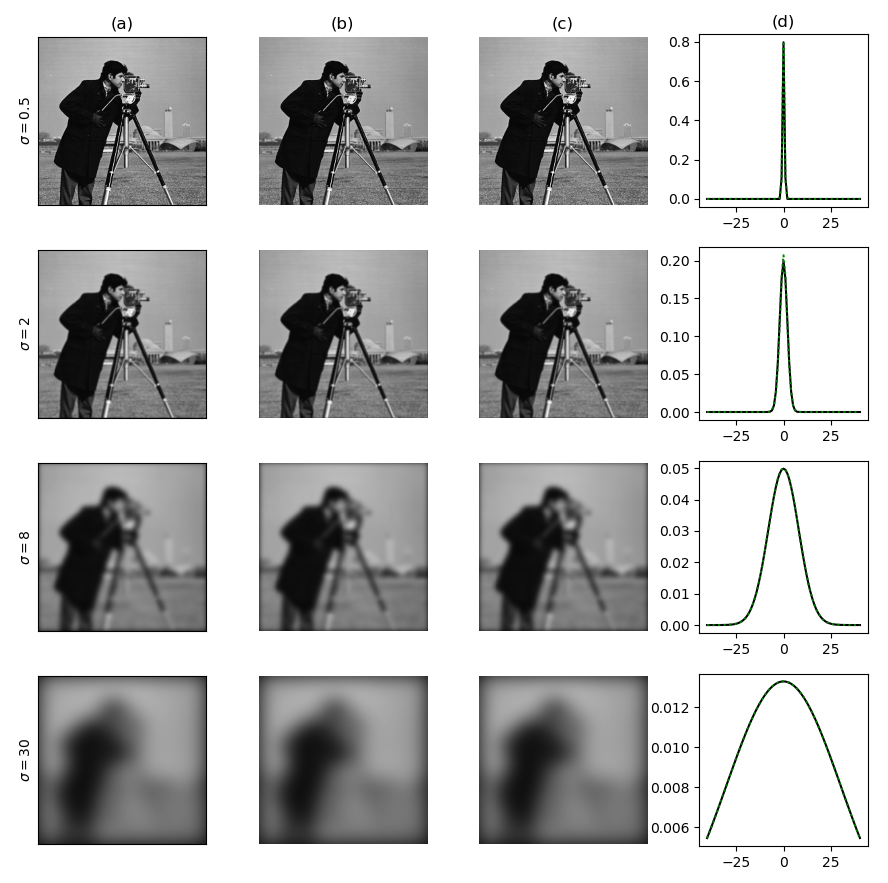
\includegraphics[width=\linewidth]{fft_gaussian_demo}
  \caption{Compatibility of Gaussian convolution strategies}
  \label{fig:fft-gaussian-demo}
\end{figure}

We also demonstrated the ``semigroup property'' of Gaussian kernel convolution.
For a large scale ($\sigma=45$) Gaussian blur ((a) - standard convolution with sampled kernel, (b) FFT with sampled kernel, (c) FFT with discrete kernel), the top row is one round of Gaussian blur with $\sigma=45$ and the bottom row is two progressive passes of Gaussian blur ($\sigma_1 = 10, \sigma_2 = 35$). The mean squared error and mean absolute error between the one-pass and two-pass versions are outputted in \cref{tab:gaussian-mae-mse}. Code for this demo can be found in \texttt{hfft.semigroup\_demo}.
The discrete kernel performs very slightly better than the sampled versions. We originally attempted
this demonstration with a much larger sigma (say $\sigma=150$) and multiple iterations, but unfortunately multiple passes cause the ``noise'' from zeroing out around the boundaries to become very noticable after several iterations. Here, we've opted to crop out a radius of pixels from around the edges equal to the standard deviation of the Gaussian before we calculated the MAE or MSE, to reduce noise from the border.

\begin{table}
  \caption{MSE and MAE of One-pass vs. Two-pass Gaussian Blur}
  \centering
  \begin{tabular}{|c|c|c|}
    \hline
    convolution implementation   & MSE & MAE \\
    \hline
    spatial convolution, sampled kernel (A) & 0.00054426 & 0.02015643 \\
    FFT convolution, sampled kernel (B) & 0.00055205 & 0.02029916 \\
    FFT convolution, discrete kernel (C) & 0.00054406 & 0.02015336 \\
    \hline
  \end{tabular}

\label{tab:gaussian-mae-mse}
\end{table}

%%REMOVED SEMIGROUP FIGURE, not worth it, just show data

%\begin{figure}
%  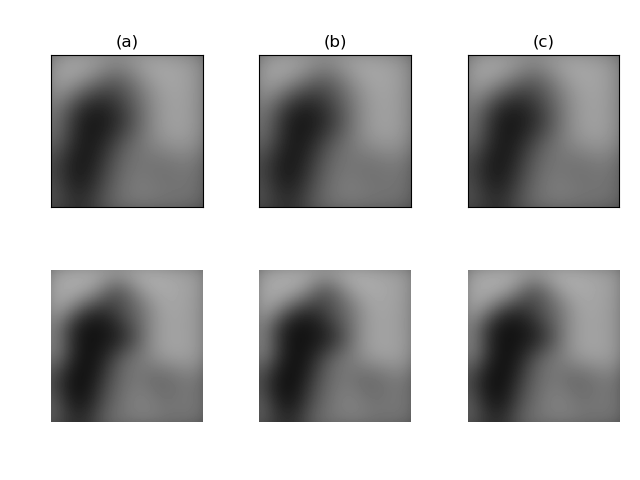
\includegraphics[width=\linewidth]{semigroup_demo}
%  \caption{Iterative Gaussian blur}
%  \label{fig:semigroup-demo}
%\end{figure}

We further confirm the commensurate nature of Gaussian blur techniques by comparing the three techniques on a placental image and using each to calculate Frangi targets. The code can be found in \texttt{hfft\_accuracy.py}. In \cref{tab:mse-G-sigma-0.3,tab:mse-F-sigma-0.3,tab:mse-G-sigma-5,tab:mse-F-sigma-5} we compare the mean squared error of a single image blurred (A) with standard spatial convolution, (B) with FFT sampled Gaussian kernel, and (C) with the discrete kernel. We see that the standard convolution and discrete convolution are very similar, while the sampled discrete Gaussian is off by two orders of magnitude, but still reasonably small. We further confirm these by viewing the grayscale intensity of the image from 0 to 1 and the Frangi targets themselves across an arbitrarily chosen horizontal cross section of the image
\cref{fig:cross-sec-demos}, the peaks of the Gaussian blurred image all still occur at the same places, as do the Frangi responses. We repeated this procedure up to $\sigma=90$ and found a situation similar to $\sigma=5$; it was only in very small scales where there was any noticeable difference at all.


\begin{table}
  %\parbox{.45\linewidth}{
    \caption{MSE of Gaussian Blurs ($\sigma=0.3$)}
    \centering
    \begin{tabular}{|c|c|c|c|}
      \hline
      &  A & B & C \\
      \hline
      A & -  & 1.296e-03 & 6.772e-06 \\
      B & -  & - & 1.247e-03 \\
      C & -  &  - &  - \\
      \hline
    \end{tabular}
    \label{tab:mse-G-sigma-0.3}
  %}
\end{table}
\begin{table}
      \caption{MSE of Frangi Scores $\sigma=0.3$}
  %\parbox{.45\linewidth}{
    \centering
    \begin{tabular}{|c|c|c|c|}
      \hline
      &  A &  B         & C \\
      \hline
      A &  - &  4.256e-06 & 5.537e-08 \\
      B &  - &  -         & 4.337e-06 \\
      C &  - &  -         &  - \\
      \hline
    \end{tabular}

    \label{tab:mse-F-sigma-0.3}
  %}
\end{table}



\begin{figure}
  \centering
  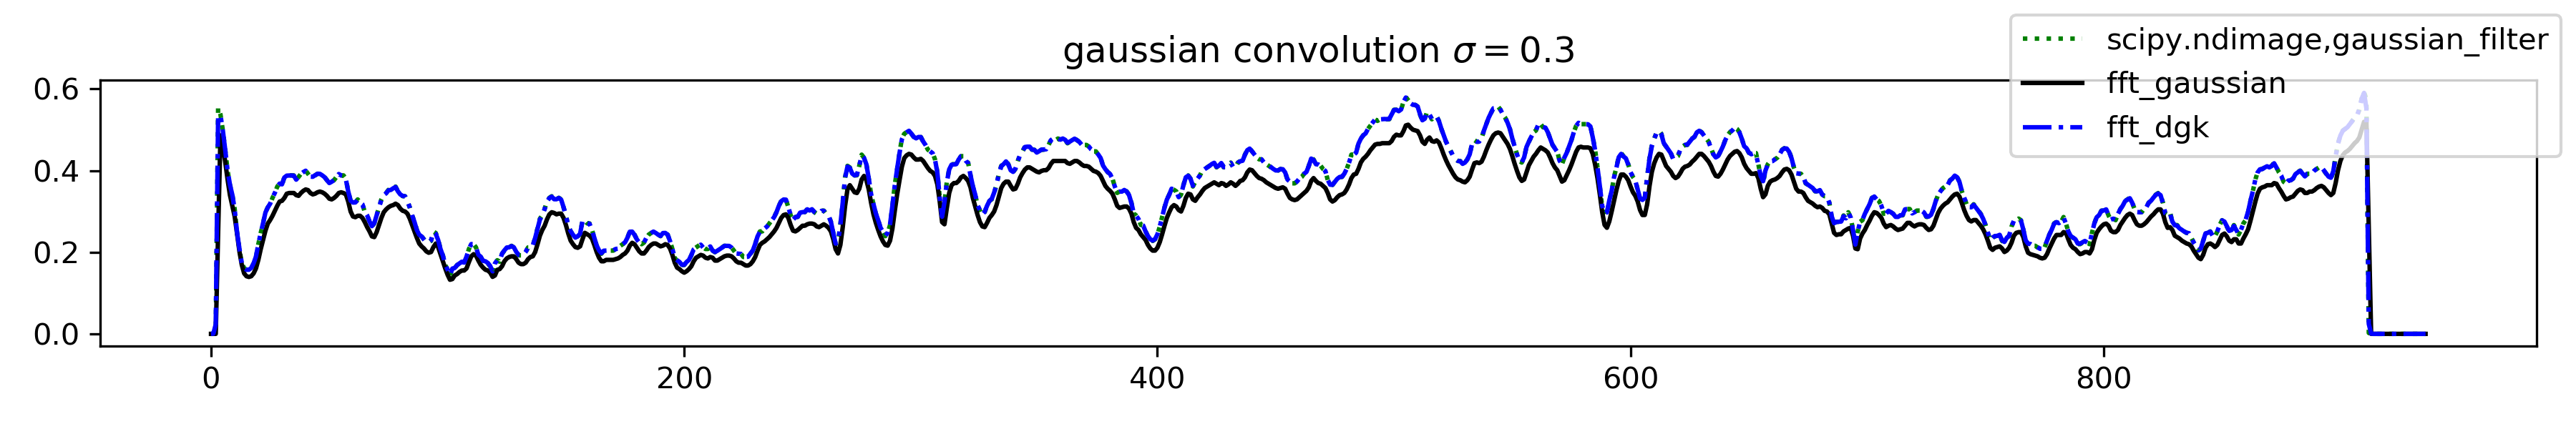
\includegraphics[width=\linewidth]{Gslice_sigma=3} \\
  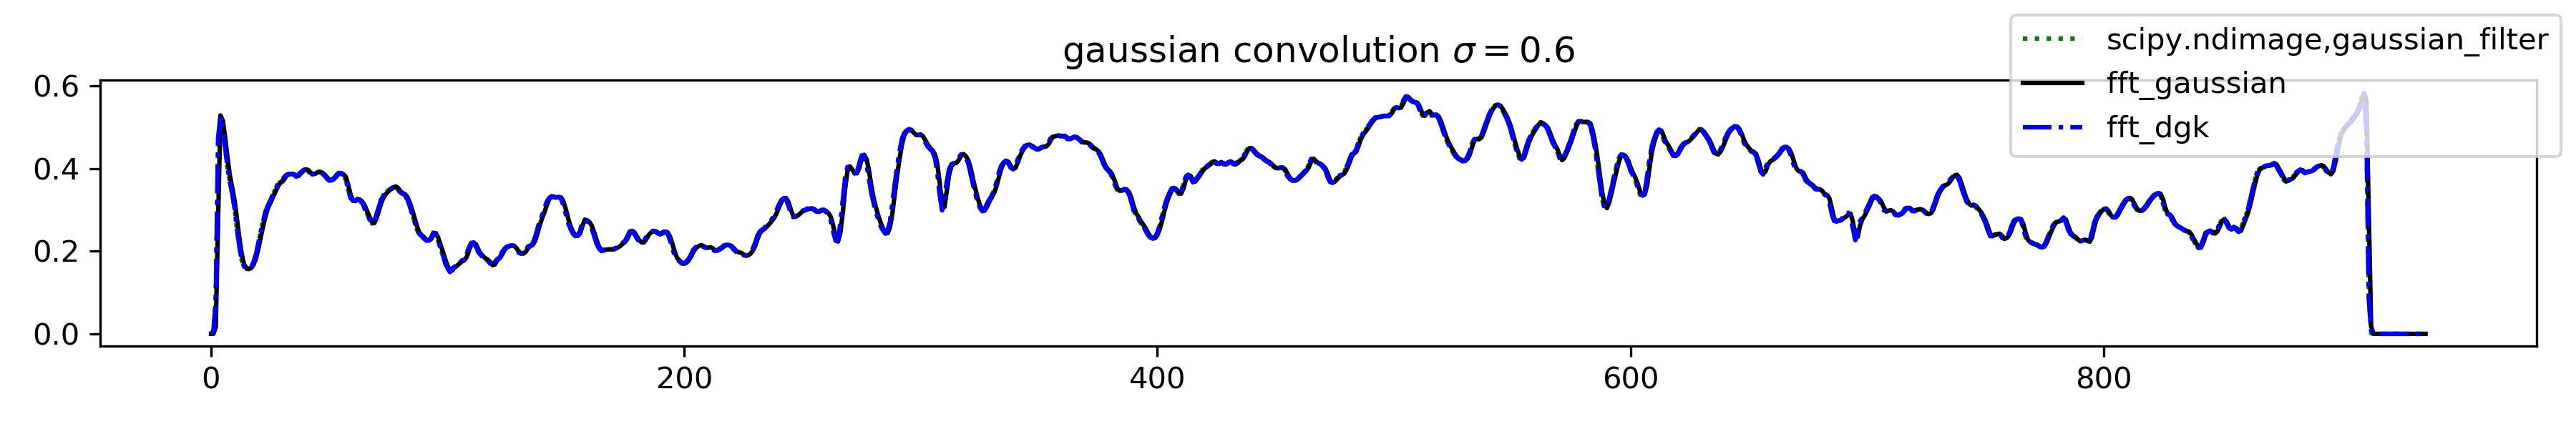
\includegraphics[width=\linewidth]{Gslice_sigma=6} \\
  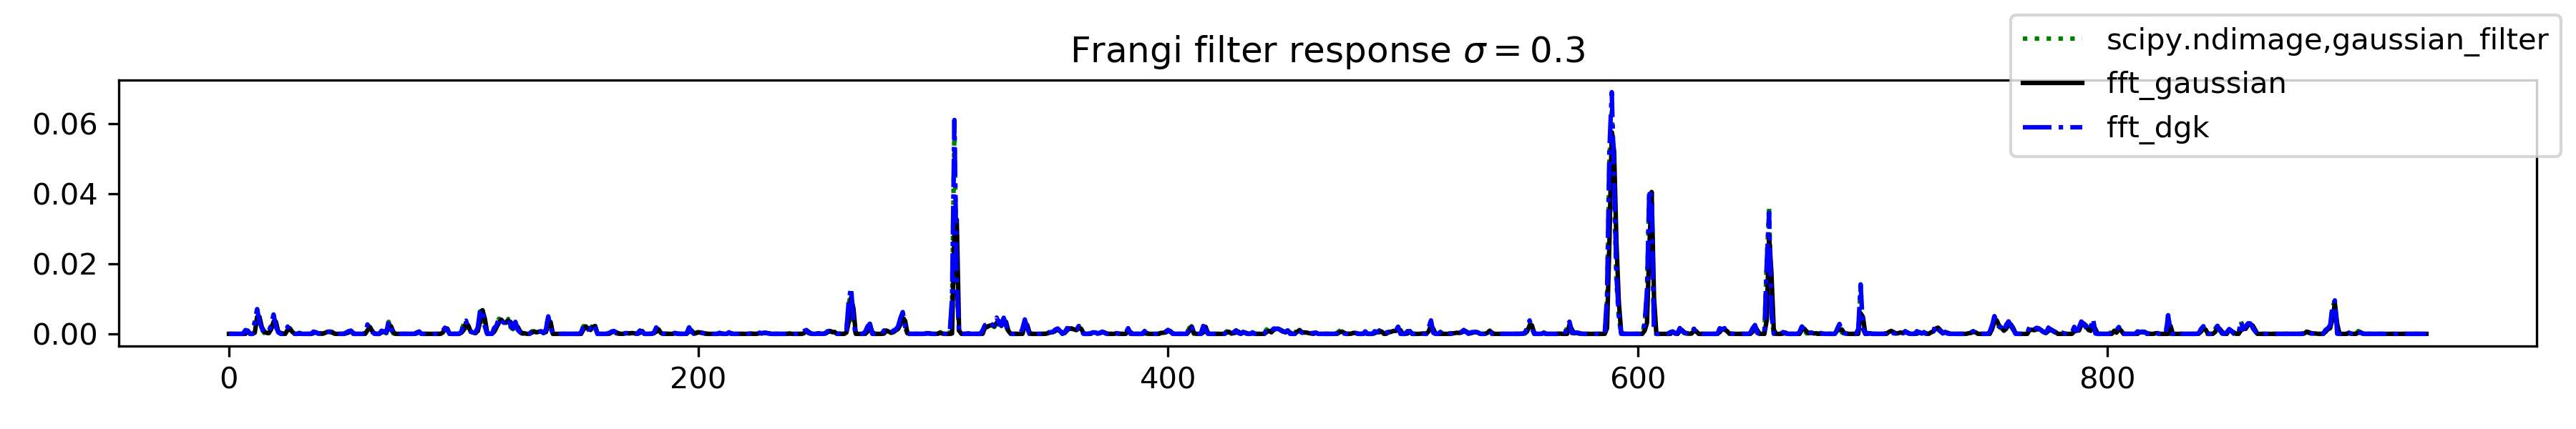
\includegraphics[width=\linewidth]{Fslice_sigma=3} \\
  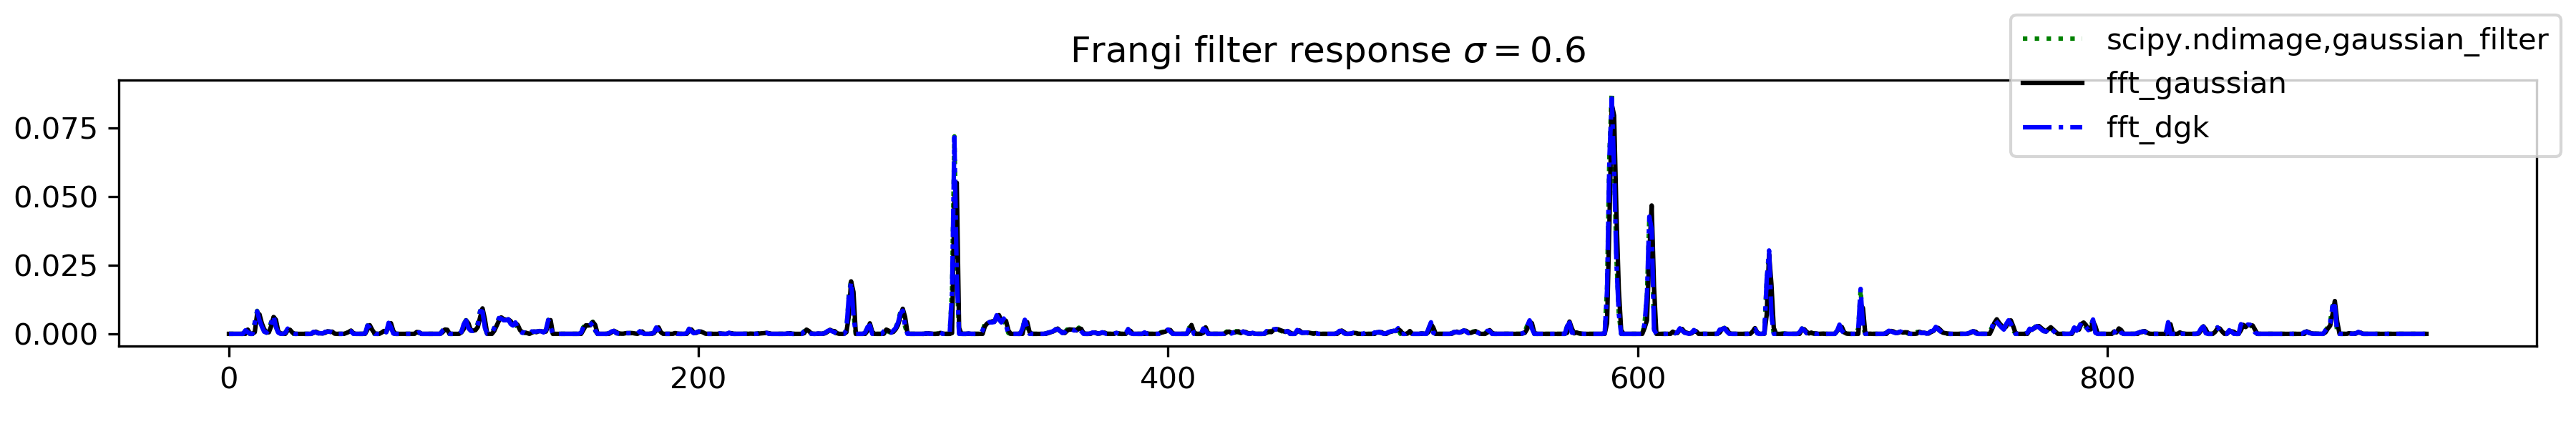
\includegraphics[width=\linewidth]{Fslice_sigma=6}
  \caption{Image cross-section of Gaussian-blurred (grayscale) placental sample}
  \label{fig:cross-sec-demos}
\end{figure}



\begin{table}
  %\parbox{.45\linewidth}{
      \caption{MSE of Gaussian Blurs of an Image ($\sigma=5$)}
    \centering
    \begin{tabular}{|c|c|c|c|}
      \hline
      &  A & B & C \\
      \hline
      A & -  &  9.012e-06 & 8.629e-09 \\
      B & -  & - & 9.031e-06 \\
      C & -  &  - &  - \\
      \hline
    \end{tabular}
    \label{tab:mse-G-sigma-5}
  %}
\end{table}
\begin{table}
   \caption{MSE of Frangi Scores $\sigma=5$}
  %\parbox{.45\linewidth}{
    \centering
    \begin{tabular}{|c|c|c|c|}
      \hline
      &  A &  B         & C \\
      \hline
      A &  - &  9.388e-05 & 8.383e-07 \\
      \hline
      B &  - &  -         & 9.599e-05 \\
      \hline
      C &  - &  -         &  - \\
      \hline
    \end{tabular}
    \label{tab:mse-F-sigma-5}
  %}
\end{table}

Finally, we wish to demonstrate the point of this comparison--that $FFT-based$ convolution is much faster than spatial convolution. We took a much larger sample ($2200 \times 2561$) and timed each method of convolution (average of three trials) for a large number of samples: logarithmic between $\sigma=1$ and $\sigma=128$ with 32 steps. We plot the result in \cref{fig:gconv-runtime}. It shows that the convolution time seems to at least linearly increase with the size of the kernel, whereas FFT is independent of choice of scale. This is to be expected, as convolving with a Gaussian kernel in spatial coordinates requires a greater number of calculations as $\sigma$ increases, whereas the size of the kernel does not change in our frequency space convolution.

\begin{figure}
  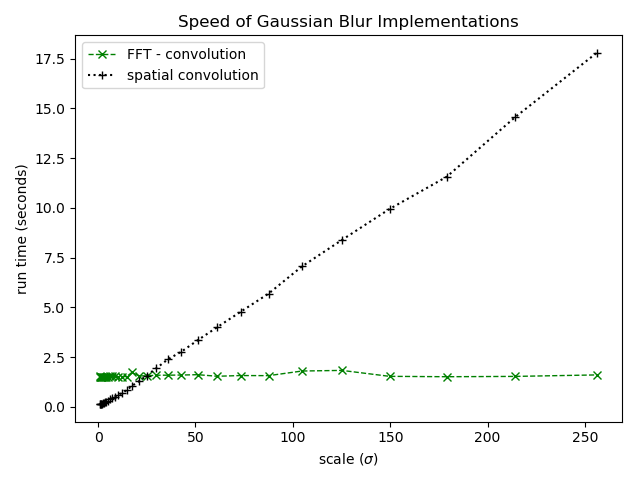
\includegraphics[width=\linewidth]{convolution-runtime-demo}
  \caption{Runtime comparison of Gaussian convolution implementations}
  \label{fig:gconv-runtime}
\end{figure}


